\documentclass[a4paper,fontset = windows]{ctexbook}
\usepackage{xifthen}
\usepackage{calc}
\usepackage{graphicx}
\usepackage{tikz}
\usepackage[user=teacher]{cexam}

\begin{document}
\chapter{基本排版程序}

 \begin{judgements}
  1.用 $v-t$ 图像表示小车的运动情况时,以速度$v$ 为\blank{纵轴}、时间 $t$ 为\blank{横轴} 建立直角坐标系,用描点法画出小车的 $v-t$ 图象,图线的 \blank{斜率} 表示加速度的大小,如果 $v-t$ 图象是一条倾斜的直线,说明小车的速度是\blank{均匀变化}的。
 
 a.*
 
 e.此题考察 $v-t$ 图象的意义,通过 $v-t$ 图象识别加速度和判断物体运动特征。

 2.某学校田径运动场 $400m$标准跑道如
 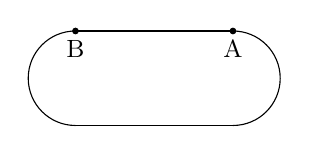
\begin{tikzpicture}
  \draw (-1,0.6)--(1,0.6);
  \draw (-1,-0.6)--(1,-0.6);
  \draw (1,-0.6) arc (-90:90:0.6);
  \draw (-1,0.6) arc (90:270:0.6);
  \filldraw (-1,0.6) circle [radius=1pt] node [anchor=north] {\small B};
  \filldraw (1,0.6) circle [radius=1pt]  node [anchor=north] {\small A};
 \end{tikzpicture}
 所示,$100m$ 赛跑的起跑点在$A$点,终点在$B$点,$400m$ 赛跑的起跑点和终点都在$B$ 点.在校运动会中,甲、乙两位同学分别参加了$100m$ 、$400m$ 项目的比赛,关于甲、
 乙两位同学运动的位移大小和路程的说法中正确的是

 \end{judgements}



\end{document}
